\section{Durchführung und Aufbau}
\label{sec:Durchführung}

Die in diesem Versuch verwendete Wärmepumpe hat den in Abbildung \ref{img:VerwendeteWaermepumpe} gezeigten Aufbau. Zu Beginn werden die Ruhedrücke und Temperaturen, sowie die spezifische Wärmekapazität des Kupfers aufgenommen. Nachdem die beiden Wasserreservoire befüllt wurden, werden die Rührmotoren angeschaltet, um die Wassertemperatur in den Reservoiren konstant zu halten. Sodann wird der Kompressor eingeschaltet und die Messreihe gestartet. Dazu werden die Messdaten der Mano- und Thermometer, sowie die Leistungsaufnahme des Kompressors im Minutentakt notiert. Die Messreihe wird beendet, wenn die Temperatur $T_\text{1}$ $50^\circ \text{C}$ erreicht hat. Für den Versuch wurde Dichlordifluormethan verwendet. \\
Wichtig ist, dass sämtliche Leitungen und die beiden Reservoire wärmeisoliert sind, um die Wärmeverluste zu minimieren.
\begin{figure}
	\centering
	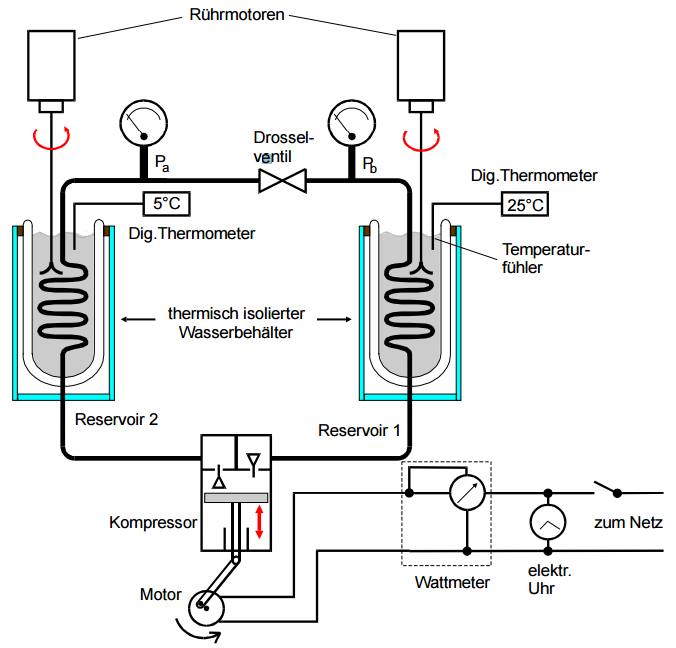
\includegraphics[height=9cm]{Versuchsaufbau.png}
	\caption{Verwendete Wärmepumpe \cite{Abb}}
 	\label{img:VerwendeteWaermepumpe}
\end{figure}
\newpage
